%========================================================================
% Modelo para elaboracao de textos academicos: TCC, dissertacoes e teses
% Elaborado pelo GISIS - Grupo de Imageamento Sismico e Inversao Sismica.
%========================================================================
\chapter{Metodologia}
\label{ch:metodologia}

Uma boa prática é iniciar a redação do trabalho (relatório, monografia, dissertação, tese) pelo capítulo de Metodologia.

Na seção de Metodologia, será descrito, de forma clara e precisa, como o seu estudo foi executado. O estilo de escrita desta seção deve parecer como se estivesse explicando verbalmente como o estudo foi conduzido, porém, usando a norma culta da língua. Evite a utilização de primeira pessoa e lembre-se de escrever no passado, uma vez que o estudo já foi executado. Organize essa seção da seguinte forma:

    \begin{itemize}
        \item Descreva o objeto de estudo: deve-se descrever a (1) origem do objeto estudado, como foi feito, onde foi encontrado, etc. e (2) suas características, seu tamanho, tecnologias utilizadas na construção, etc. É importante ter em mente que esses dados dependem da área estudada. Por exemplo, na área de Ciência da Computação é comum descrever o tamanho do software em linhas de código, seu número de módulos, qual linguagem foi utilizada na construção e quais as tecnologias envolvidas.
        \item Quando o estudo é realizado fora do ambiente controlável do laboratório, é necessário descrever o local onde o estudo foi realizado e quais eram as condições.
        \item Descreva como os dados foram coletados durante o experimento. Escreva com detalhe suficiente para que o outro pesquisador, lendo seu texto, tenha condição de repetir seu estudo.
        \item Descreva como os dados foram analisados. São indicados o(s) método(s) estatístico(s) utilizado(s), qual e como foi aplicado, e que tipo de análise foi empregada para responder cada questão da pesquisa ou testar as hipóteses do estudo.
        \item Descreva claramente a infraestrutura e configurações necessárias para seu experimento.
    \end{itemize}
    
Um recurso muito útil para esclarecer as etapas da metodologia é utilizar um fluxograma conforme o que está representado na Figura \ref{fig:FluxogramaMetodologia}.
        \begin{figure}[h]
            \vspace{0.2cm}
            \centering
            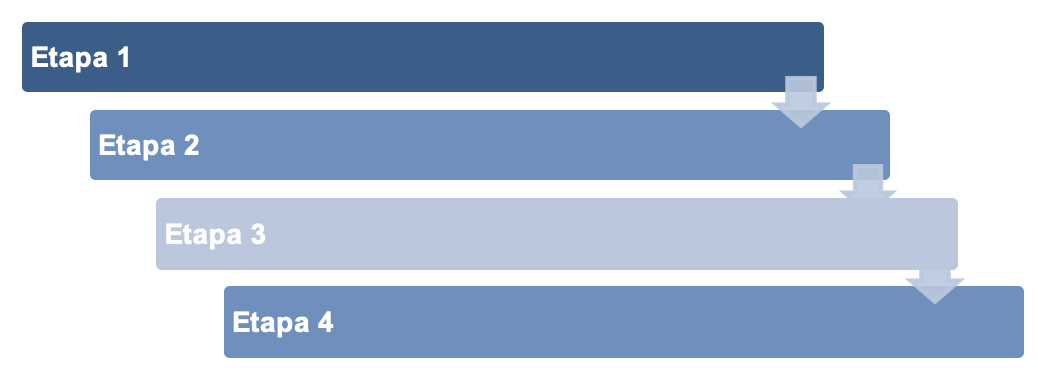
\includegraphics[width= \textwidth]{Imgs/Metodologia/fluxogramaMetodologia.png}
            \caption[Fluxograma da metodologia adotada.]{Fluxograma da metodologia adotada. Fonte: O autor.} 
           \label{fig:FluxogramaMetodologia}
            \vspace{0.2cm}
        \end{figure}